\chapter[SCP-001 黎明将至]{
	SCP-001 S. D. Locke - When Day Breaks \\
	SCP-001 黎明将至
}

\label{chap:SCP-001.when.day.breaks}

\begin{scpbox}

你发现了那条通道,正隐藏在距主干道一英里外的天然洞穴内。

无需钥匙卡,通道之门是敞开的。

这里的气味闻起来和它们一样。但愿它们已经离开了。你走的太远,你无法回头了。

一条平滑的小径从洞口向内延伸,通向站点深处。也许会有些血液或粪便 – 或是那些东西涂抹的污渍,这可说不准。所以你得小心避开。

你仍能收到求救信号,它是从昨天开始的,无论是谁 – 你祈祷他们能够生还。

你的脚步声回响在空荡走廊之中,每一步都仿佛传达自另一个世界,就好像你并非在黑暗中独行。

电梯停留在底层 – 故而你沿楼梯下行,直至B5层:Keter控制区,你穿过几个空收容室,它们曾能造成的恐惧和动荡早已不复存在。

如果你运气够好的话。

这条路将你带往大厅一侧的办公室 – 那里正是信号的来源。门没上锁,但被什么东西卡住了,你抬起脚,用尽全力踹了过去。

在你能看清屋里的事物前有个东西从你左侧的角落里冲了出来,你的第一反应是“狗”。

但它曾蛰伏在天花板上。

你躲入房间,砰地关上身后的门。此处一片漆黑,你是安全的。你脱下外套,摘掉头盔。在经历了如此之多的事情后却死于中暑将会是莫大的耻辱。

唯一的应急操作灯旋转在塑料外壳之中 - 每隔一秒便在房间中洒下暖橙色的灯光,仿佛房间本身的脉搏正有节奏地律动着。

门后随意搁置着 – 一个路障,你环顾四周,脏衣服和吃了一半的食物,尽管临近厕所,角落里却有个盛满排泄物的桶。北面墙上的气动室将向房客提供必要的生活物资。

你的路终止于房间角落某个令人作呕的泥潭,你看到了三个药瓶 - 检查发现这是三种不同的鸦片类药物,它们都是空的。

桌上有台电脑,靠近终端,你可以清楚地看到电源指示键闪烁着微弱的灯光。

你坐下,开机。

\end{scpbox}

\hr

\cl{

\Gg{紧急协议激活。删除级别保护措施。完全访问权限。}

控制。收容。保护。

\par

\par

加载中...

加载中..

加载中...

加载中..

加载中...

加载中......

}

\begin{scpbox}
你听到门外传来了脚步声,一步步愈发沉重,下一步又接踵而至。
\end{scpbox}

\cl{

加载中...

加载中..

加载中...

加载中..

加载中...

加载中..

加载中...

加载中..

加载中...

正在验证...

..

...

}

\begin{scpbox}
黑影由地板和门边的缝隙悄然渗入,被光线映照地轮廓分明。
\end{scpbox}

\cl{

..

...

..

正在验证...

..

...

..

...

..

正在验证...

..

...

}

\begin{scpbox}
你紧张地屏住呼吸等待着,希望它只是路过。然而你的心跳此刻在你自己听来,却震耳欲聋地暴露了你的位置。
\end{scpbox}

\cl{

请等待...

..

...

..

..

...

请等待...

..

...

..

请等待...

..

...

..

}

\begin{scpbox}
阴影消失了,你的呼吸松懈下来,正在这时,屏幕亮了起来……
\end{scpbox}

\par

\cl{

打开文件

\Gg{🔥 自动化安全系统通知代码235(ASSN-235) 🔥}

检索SCP-001文件当前迭代时出错,您正在查阅版本\#3,可滑动至页面底部查阅较新版本。

}

\tred{开启文件:SCP-001 修订版\#3/12:(1) 音频文件}


\Gg{\bb{修订版 \#3/12 更新于1312日前}}

\hr

\begin{figure}[H]
	\centering
	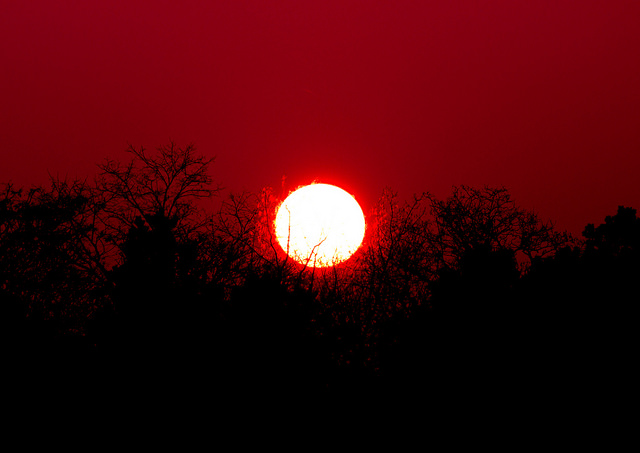
\includegraphics[width=0.5\linewidth]{images/SCP.001.when.night.breaks.jpg}
	\caption*{SCP-001激活后数分钟,拍摄者未知。}
\end{figure}

\bb{项目编号:}SCP-001

\bb{项目等级:}Apollyon\footnote{译注:abad,希伯来语意为破坏者,希腊语译为apollyon,英语译为abaddon,指圣经启示录中的地狱使者亚巴顿,又称无底坑的使者。}

\bb{特殊收容措施:}由于其性质,SCP-001无法被收容。SCP-001事件幸存者将驻扎在安全设施中并彼此保持联系,鼓励人员采取任何可行的手段前往Site-19。

希望进行户外活动的幸存者必须保证周身覆盖防护服;最好是多层防护,应尽可能避免徒步旅行,城市 – 也指通常意义上的人造建筑可提供最大程度的庇护,需规避树木繁盛区,空乘是所有出行方式中的最优选择。

暴露于SCP-001的人员将被视为损失,受连累者将被遗弃,请不要尝试安乐死。

应不惜一切代价避免SCP-001-A组成规模庞大的集群,已证实电导武器在固定情况下有一定作用,故可用于自卫,燃烧器也可正常使用,迄今为止,冷冻弹药是最有效的。

测试显示SCP-001-A是相对安全的可消耗品,但只能被视为没有其他选择的情况下的最后手段。由于SCP-001-A可在消化系统中重构,因此短时间内仅能消耗少量,以防止堵塞。

驻扎于Site-19的人员从事有关世界殖民化的研究,载具经过专门设计,内部不得被光线穿透。

\begin{scpbox}

\begin{scpbox}

对于那些失去了家人,或者上帝啊,失去了孩子的人们 – 我对此深感,深感遗憾。但你必须坚持下去,不要让他们白白死去,我们还有时间。

人类仍可能拥有未来,到Site-19来,我们需要尽可能多的援助。

学会拥抱黑暗,朋友们,我们惧怕光明。

\hr

\hfill - \ii{The Administrator}

\end{scpbox}

\end{scpbox}

\bb{描述:}SCP-001是在事件[系统错误]\ii{数据丢失:ec172,请联系系统管理员。}后对于太阳的编号。此次事件发生二十四小时内造成约68亿人类伤亡。SCP-001的影响似乎不是经由紫外线产生,而是暴露于可视光谱(~390至100nm)导致。即使身在月光下也同样如此。

当活体接触太阳产生的可见光时,将从接触点处开始液化,效果持续扩散,直至整个生物体完全转化。从外观上来看,同蜡融化类似。转化时间很大程度上取决于生物体的暴露程度和其大小。尽管发生了这种重组,生物体也不会死亡。

转化完成后,这些生物体(SCP-001-A)将呈凝胶状,它们会尝试活动,尽可能使自己固定在可令人联想起先前样貌的形态,这种努力可取得一定程度的成功。

植物通常保持物理惰性,但仍能够进行光合作用并产生氧气,可飞行的生物丧失飞行能力,动物具有意识,在未被吸收至集群的前提下,行为与往日无异。人类则保有少许智慧和记忆。

暴露于SCP-001的生物性异常受到同样的影响,曝光可抹消其曾表现出的全部异常。

由于它们的物质组成,SCP-001-A个体可通过彼此接触进行分子水平上的联接和混合,这似乎不会对个体造成任何痛苦和伤害,但组成的体积可抑制其运动。自SCP-001-A事件以来,大多数个体已集聚为这样的集群,似乎不存在最大融合上限。

融合后的生物质是无定形且混沌的,集群生物将在半液态中转换形态 – 其中肢体和身体质量将在短时间内周期性升高,随后恶化并被另一种生命形态纳入。

集群个体将使用它们的附属物来移动自身的质量,多数情况下它们会使用组织成分构建伪足,并以类似变形虫的方式拖动自己。

\cl{\red{
+打开附件:音频日志 \\
... \\
... \\
... \\
授予访问权限。
}}

\begin{scpbox}

当你打开文件时,扬声器中发出了刺耳的静电噪音,扰乱了房间的静谧,你措手不及,心跳加快。也有些噪音来自于调节麦克风。

沉默转瞬而逝:

\end{scpbox}

\begin{scpdialog}
“咳咳,这里是Logan Igotta博士,级别,嗯,三级研究员。”
\end{scpdialog}

\begin{scpbox}
她的声音有些颤抖,以至于听起来没有那么专业。她停顿片刻,深吸一口气,而后继续说道。
\end{scpbox}

\begin{scpdialog}
“由于Site-46拥有几个传染性信息危害 – 所以我们,我们启用停电协议将 – 将其余网络切断了,因此我们将使用新信息通道来传递现状。

从好的一面来说,我们实际上还能接收到来自其他几个站点的信息,似乎有相当数量的人这么做了,有些计划突破19,有些正试图冲击As,也有些,和我们一样,只是简单地等待时机。我们的站点暂时封闭,我们还没准备好旅行,至少现在还没有。
\end{scpdialog}

\begin{scpbox}
她叹了口气。
\end{scpbox}

\begin{scpdialog}

“几天前我们……遭遇了一次收容失效,一台类人型机器人失控了,这王八蛋放跑了半打,半打Keters。

在像碗浓汤似的崩溃前,它们没能跑出隧道五英尺远。我 – 我看着它们倒在凸轮上。

没过多久它们又重新站了起来。”

\end{scpdialog}

\begin{scpbox}

她再度停了下来,念诵着你难以理解的呓语 – 在你能够继续听见明确无误的语句之前。

她几不可闻地呼气。

\end{scpbox}

\begin{scpdialog}
“啊.……好,好多了,恰好在指定吸烟区;但是到底发生了什么,嗯?
\end{scpdialog}

\begin{scpbox}
她清了清喉咙。
\end{scpbox}

\begin{scpdialog}
“指挥官Anand穿戴整齐,第二天便去了镇上,试图去赶他们。事态没什么好转,可怜的混蛋。不过我们确实学到了一两件事。”
\end{scpdialog}

\begin{scpbox}
停顿,喘息。
\end{scpbox}

\begin{scpdialog}

“只有少数几个人离开了这里,我躲在办公室里,Herry和Phillips主任在营房的某处,Clyde和几个D级把自己锁在了军械库里,和Ari一起。

我真该去看看她要做些什么的。”

\end{scpdialog}

\begin{scpbox}
片刻间她哑了声 – 你听到无线电喋喋不休的嗡嗡声。
\end{scpbox}

\begin{scpdialog}
“嘿,嗯,你在那儿怎么样?”
\end{scpdialog}

\begin{scpbox}
一个声音回应了她,是个极为夸张、语调嘲讽的男声。
\end{scpbox}

\begin{scpdialog}
“我现在在这也就是照料 - !我要你知道我 - !呃,唔。”
\end{scpdialog}

\begin{scpbox}
Logan开枪还击。
\end{scpbox}

\begin{scpdialog}
“谁?谁呢 – 把它关掉,该死的我要跟她通话。”
\end{scpdialog}

\begin{scpbox}
另一端则传来喧哗声,收音机易了手。温柔而关切的声音正呼唤着。
\end{scpbox}

\begin{scpdialog}
“宝贝,怎么了?”
\end{scpdialog}

\begin{scpbox}
Logan回应道。
\end{scpbox}

\begin{scpdialog}
“没事 – 没事 – 什么都没有。”
\end{scpdialog}

\begin{scpdialog}
停顿,喘息。
\end{scpdialog}

\begin{scpdialog}
“我只想尽快确认一下。”
\end{scpdialog}

\begin{scpbox}
Ari恳求着。
\end{scpbox}

\begin{scpdialog}
“我很好,宝贝,真的,我能照顾好自己。”
\end{scpdialog}

\begin{scpbox}
咯吱声 – Logan转过座椅。
\end{scpbox}

\begin{scpdialog}
“不,不,我知道,我明白,我无能为力,我知道来到这儿对你来说很不容易……”
\end{scpdialog}

\begin{scpdialog}
“……一切事情都——”
\end{scpdialog}

\begin{scpbox}
Ari打断了她的话。
\end{scpbox}

\begin{scpdialog}
“嘿,你告诉我你戒烟了。”
\end{scpdialog}

\begin{scpbox}
短暂的噪音,也许是Igotta试图掐灭她的香烟。
\end{scpbox}

\begin{scpdialog}
“哦!呃……不!不,当然的,我的意思是,我戒烟了。”
\end{scpdialog}

\begin{scpbox}
Ari似乎并不相信。
\end{scpbox}

\begin{scpdialog}
“我想你并不需要担心我,我一直很干净,甚至这几个月都没想过碰致幻药。相信我。

无论如何,既然你想知道,我没事。小伙子们正围在扑克牌边,我和笔记本一起窝在角落里。”
\end{scpdialog}

\begin{scpbox}
你可以听到Igotta开玩笑似的笑了笑。
\end{scpbox}

\begin{scpdialog}
“亲爱的!在这样的时刻还想着要写首关于你我之间永恒爱恋的十四行情诗?我受宠若惊。”
\end{scpdialog}

\begin{scpbox}
Ari笑着回答。
\end{scpbox}

\begin{scpdialog}
“一首挽歌,如果我现在无法让自己沉浸在某事之中,一定会发疯的。”
\end{scpdialog}

\begin{scpdialog}
“我明白,嗯,我会尽快带你回来的。

我爱你。”
\end{scpdialog}

\begin{scpbox}
Ari回答。
\end{scpbox}

\begin{scpdialog}
“我也爱你,宝贝。”
\end{scpdialog}

\begin{scpbox}
片刻的寂静,通讯中止,而后又是一声几不可闻的叹息。
\end{scpbox}

\begin{scpdialog}
“我们只剩下这些人了,其他的要么在事件中丧生,或是死于收容失效。主任命令我们原地待命,继续盯紧凸轮 – 那里面的还有设施附近的,001跳跃在我们的门前,天知道我们这儿还锁了什么东西。

电力仍在运转 – 我们还能维持相当长的时间 – 而且这里有足够多的物资能够维持数年,我们能过得很好。”
\end{scpdialog}

\begin{scpbox}
停顿,喘息。
\end{scpbox}

\begin{scpdialog}
 “一切都会好起来的。” 
\end{scpdialog}

\begin{scpbox}
传输结束前,她等待了几拍。
\end{scpbox}

\hr

\tred{开启文件:SCP-001 修订版\#5/12:附加事件报告}

\hr

\Gg{\bb{修订版 \#5/12 更新于1202日前}}

\begin{figure}[H]
	\centering
	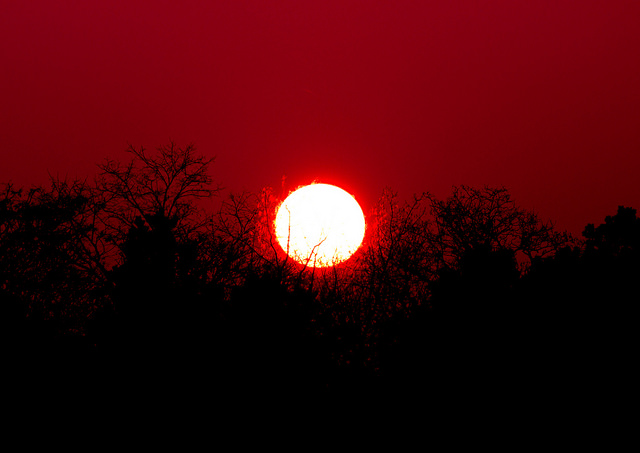
\includegraphics[width=0.5\linewidth]{images/SCP.001.when.night.breaks.jpg}
	\caption*{SCP-001激活后数分钟,拍摄者未知。}
\end{figure}

\bb{项目编号:}SCP-001

\bb{项目等级:}Apollyon

\bb{特殊收容措施:}\red{未提交更改。信息崩溃。}

\bb{描述:}\red{未提交更改。信息崩溃。}

\cl{\red{
+打开附件:事故报告-001.1\\
...\\
...\\
...\\
授予访问权限
}}

\begin{whitebox}[left=2pt, right=2pt, top=2pt, bottom=2pt]

他们一直坐在那里,呼唤并乞求我们走到外面去。噪音引来了更多人。这样庞大的一个集群,我敢肯定至少有几十个人,天晓得里面混杂了多少动物。尖叫、抱怨、怒吼和咆哮声此起彼伏,简直比地狱更响亮。最糟糕的是令人恶心的呻吟声 – 就好像他们真的在享受似的。

他们只要知道我们还在这里,就不会离去。

我们设法说服了一个D级出去看看 – 看他能不能把它们引开,他的计划令人惊讶 – 他只要了一把手枪,和一颗子弹。他走到它那儿去,随即它捉住他试图掀开他的面具,他设法将枪口抵住下巴然后扣动扳机。我想他很幸运。

他踉跄地跌倒在地,它滑进了他的防护服,撬开面罩,从内部开始将他撕裂。

他回来了;开始转化 – 曾是他身体的凝胶从衣服中滴落,尖叫尖叫尖叫。

它们甚至不让我们寻死。

主任有个计划,他的办公室里有个逃生隧道,站点下方的电车可以将我们带到一个安全屋 – 我们应该可以从那里起步,前往Site-19。

\end{whitebox}

\hr

\tred{开启文件:SCP-001 修订版\#8/12 一(1)附件}

\hr

\Gg{\bb{修订版 \#8/12 更新于1200日前}}

\begin{figure}[H]
	\centering
	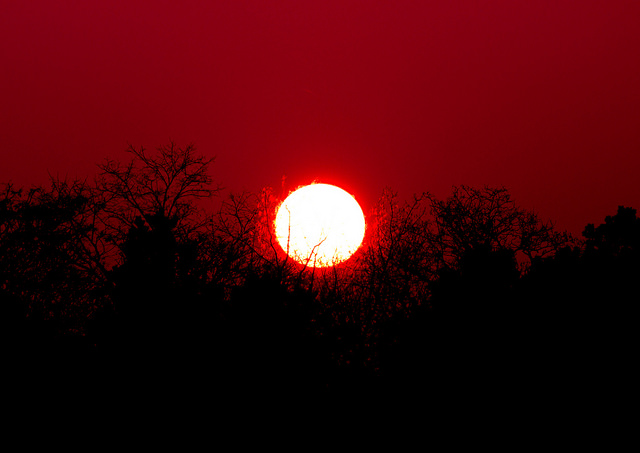
\includegraphics[width=0.5\linewidth]{images/SCP.001.when.night.breaks.jpg}
	\caption*{SCP-001激活后数分钟,拍摄者未知。}
\end{figure}

\bb{项目编号:}SCP-001

\bb{项目等级:}Apollyon

\bb{特殊收容措施:}\red{未提交更改。信息崩溃。}

\bb{描述:}\red{未提交更改。信息崩溃。}

\cl{\red{
+打开附件:音频文件\\
...\\
...\\
...\\
授予访问权限
}}

\begin{scpbox}

你第一次看到她的样貌,Igotta博士坐在你现在所处的地方,神情痛苦,双眼布满血丝,胸口处晕染着大而潮湿的黑红色。

她颤抖而短促地呼吸着,嘴唇翕动,似乎是在说话,声音却哽咽在了喉咙里。她垂下头,无声地啜泣起来,一分钟后,她设法克制住自己:

\end{scpbox}

\begin{scpdialog}

“我,我 – 我们,电 – 电车……

在隧道里,从天花板流淌下来,拖动,拖动他们进入,光 – 光剥开他们的衣服,和,和 – 和……”

\end{scpdialog}

\begin{scpbox}

她将手伸入胸前的口袋,掏出半截断指,断口下方可清晰地看到结婚戒指的暗淡光泽。她紧紧握着它,捧在手心里,拇指摸索着闪烁的金属。

她近乎永恒地呆坐着,反复低声道歉,乞求宽恕,看起来失魂落魄。片刻后她抬起头来,发现自己还在录音,好像回归了现实;她将断指塞回口袋,前倾身体,像是要关闭摄像机,但是这时一台收音机发出了声音。

它播放了几秒白噪音,而后突兀地传出了令你万分紧张的声音。

\end{scpbox}

\begin{scpdialog}
“Logan?”
\end{scpdialog}

\begin{scpbox}
那几乎是Ari的声音,然而那声音已经受到影响、如肠鸣音一般。Logan错愕地张开嘴,脸庞血色尽失。
\end{scpbox}

\begin{scpdialog}

“你在哪儿?为什么我回不到里面去?

你在吗”?

\end{scpdialog}


\begin{scpbox}
Logan从办公桌下捡起一部手持式收音机,她的手有些颤抖,那东西不断恳求着她;不成人声的嗓音让你倒尽胃口。
\end{scpbox}

\begin{scpdialog}
“宝贝,没关系,\ii{我}没事,真的。

这是个明亮而阳光灿烂的好日子,你却无所事事地虚度光阴。”
\end{scpdialog}

\begin{scpbox}
Logan泪流满面,手指盘旋在呼叫按钮上方。曾是Ari的东西用一种深沉而湿润的声调呼吸并说话。
\end{scpbox}

\begin{scpdialog}
“多么美丽而澄澈的蓝天 – 和那天一模一样,你还记得吗?”
\end{scpdialog}

\begin{scpbox}
Logan用她空闲的手拿起一支烟,而后划着火柴。她哆嗦着手指两次尝试点燃烟头却失败了。她在心底默默宣誓,第三次点燃香烟,吸了四分之一。曾是Ari的东西继续说:
\end{scpbox}

\begin{scpdialog}
“这太完美了,和我一直梦想着的一模一样,你的计划真是精巧,我从未像此刻这样感受到爱。”
\end{scpdialog}

\begin{scpbox}
Logan开始摇晃。
\end{scpbox}

\begin{scpdialog}
“甚至有乐队演奏我们的歌谣……”
\end{scpdialog}

\begin{scpbox}
它开始歌唱。
\end{scpbox}

\begin{scpdialog}
\ii{“我感觉很好,以这特殊的方式}

\ii{我坠入爱河,这是个阳光明媚的好日子”}
\end{scpdialog}

\begin{scpdialog}
Logan将收音机丢出房间,它在某处磕碎了屏幕,但仍在运作 – 你仍能听到那东西的歌声。
\end{scpdialog}

\begin{scpdialog}
\ii{“好日子,阳光明媚的好日子}\\
\ii{好日子,阳光明媚的好日子”}
\end{scpdialog}

\begin{scpbox}
随着无线电慢慢消逝,越来越多的声音齐声合唱,几个,几十个,乃至更多,他们放声歌唱,直到收音机仁慈地沉寂下去,Logan从她的椅子上跳起来冲了出去,你可以听到她在屏幕外呕吐。视频画面定格在空座位上,过了几分钟,她返回并关掉了摄影机。
\end{scpbox}

\hr

\tred{等等,哪里不对。}

\begin{scpbox}

有种挥之不去的、却又似妄想的感觉包裹着你,你正被监视。你戒备地睁大眼睛,尽管视线从显示器处移开后需片刻来适应黑暗,应急灯光扫过房间,将阴影拉伸扭曲地面目全非。这时,你发现了它。

在那儿,在那角落中。

它正从泥潭中爬出。

时间在这一刻放缓,一双手,涂满了遍布整个设施的黑色粘液,撑在了令人作呕的泥潭两侧,仿佛地板下方的东西正努力支撑,试图将自己的身体抬升起来。

不成人形。

头部随之而来,从粪便中上升,乱蓬蓬的毛发遮盖了它的脸,不明液体肆意横流,它转向你的方向。

它在角落中注视着你,而后再次沉入黑暗。

应急灯光再次穿过房间,扫射着泥潭,它看起来和方才别无二致。

\end{scpbox}

\tred{开启文件:SCP-001 修订版\#9/12 一(1)附件:}

\Gg{\bb{修订版 \#9/12 更新于986日前}}

\hr

\begin{figure}[H]
	\centering
	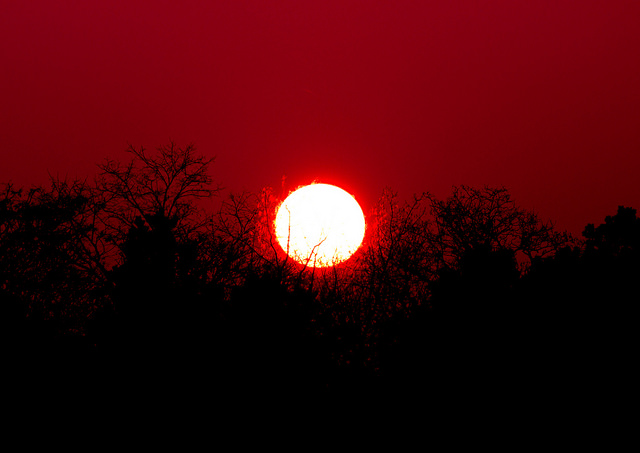
\includegraphics[width=0.5\linewidth]{images/SCP.001.when.night.breaks.jpg}
	\caption*{SCP-001激活后数分钟,拍摄者未知。}
\end{figure}

\bb{项目编号:}SCP-001

\bb{项目等级:}Apollyon

\bb{特殊收容措施:}

\bb{描述:}\red{未提交更改。信息崩溃。}

\cl{\red{
+打开附件\\
...\\
...\\
...\\
授予访问权限
}}

\begin{scpbox}
Igotta博士的身影出现在显示器上,她看起来消瘦了,大张的双眼遍布血丝。桌面上搁着一把刀,一只碗,一页表面泛黄的马尼拉信封。

上面叠着一卷染血的羊皮纸。
\end{scpbox}

\begin{scpdialog}
“虽然我们身处基金会,并且面临了这些事情,但我一直认为我们能够保持控制与收容,我们将隐匿于黑暗之中 - 令人类在光明的大道上蓬勃发展。

Site-19的通讯上月起中断了,我越来越难以找到理由坚持下去 – 尤其是,在失去了……”
\end{scpdialog}

\begin{scpbox}
她抓起刀,犹豫了片刻。
\end{scpbox}

\begin{scpdialog}
“那些声音一次又一次地在我脑海中盘旋飘荡,我时常回忆起隧道中的那天,一切事情都发生了。我已经回去过几次了,只是为了能再次听到她的声音。

但这是错误的,门那边的东西 – 不是她,她再也不会回来了。那声音听起来很像她,它也知道她所知道的一切,但它不再是她了。这光 – 它夺走你的身体,偷窃你的思想。

但你的灵魂呢?”
\end{scpdialog}

\begin{scpbox}
说到这儿,她将刀片压入左手掌心,因疼痛而抽搐。你看着她握紧拳头,令血液流入碗底
\end{scpbox}

\begin{scpdialog}
“如果这样做……能让我寻回失去的,光线无法企及之物;我会回来更新的。现在我说完了。”
\end{scpdialog}

\hr

\tred{开启文件:SCP-001 修订版\#17!24ATA 错误}

\hr

\Gg{\bb{修订版 4847/3RR0R 更新于985日前}}

\begin{figure}[H]
	\centering
	
\includegraphics[width=0.5\linewidth]{images/SCP.001.when.night.breaks.2.jpg}
	\caption*{它是多么温暖。}
\end{figure}

\bb{编号。 }伤害。

\bb{项目。 }Apologize

\bb{特殊收容措施:}SCP-001\bb{不应}被收容,SCP-001事件幸存者将驻扎在安全设施中并永远无法彼此保持联系,鼓励人员\bb{克服自身,停止思考他们所知之事。}

\bb{你不可能永远隐匿此处,吾爱。}

暴露于SCP-001的人员将\bb{不可}被遗弃,我没有要求你救我,这不是你所做的选择。 请\textsuperscript{
不要不要不要不要不要不要不要}尝试安乐死。

已证实电导武器\bb{为什么?}在固定情况下有一定作用。\bb{你无法忍受我变得更好。}燃烧器\bb{如同瘙痒。}迄今为止,冷冻弹药是最有效的。

驻扎在Site-19的人员将\bb{不遗余力,我也是,永远不会太晚,宝贝。}

\bb{描述:}SCP-001是\bb{我们终获自由后}对于太阳的称谓,其影响是瞬时的,\bb{将将你从所有痛苦中解放, 直至你将我撕裂。这种变化看起来很吓人,我明白,}尽管经历了这种充足,但你\bb{不会死。}

\bb{我保证。}

由于它们的物质组成,SCP-001-A个体可通过彼此接触进行分子水平上的联接和混合\bb{并最终以这种形态存在}。这不会造成\bb{任何痛苦}。自SCP-001-A事件以来,大多数个体已集聚为这样的集群,似乎不存在最大融合上限。\textcolor{white}{不要担忧}

所得的生物质是\textsuperscript{美}\bb{丽}\textsubscript{的},集群中的生物体将在其内部和周围游移,\textsubscript{进入}\textsuperscript{分离}\textsubscript{进入}\textsuperscript{分离}\textsubscript{进入} - 其中肢体和身体部分都将转移 \bb{永不放弃}。 \textsubscript{万物归一} 随后恶化并被另一种生命形态纳入。

集群中的个体仅是想要再度靠近你。

如此努力。\\
\small{让我进入}

\Gg{\bb{带我回去}}

\begin{scpbox}

附有一个视频文件,打开它,你将看到它拍摄者你所身处的房间,画面似乎来自一个设置在房间角落的监控摄像头。环境十分昏暗,但你可辨认出Igotta博士,躺在远处墙边堆放的衣物上。

她在睡眠中不安地扭动身体,似乎正承受着折磨和伤害。她辗转反侧,嘟囔着无意义的音节。

摄像头抖动,微微向上抬起,而后再次重点关注她。

它开始缓慢靠近。

扬声器开启;你听到了轻而平缓的呼吸,随着摄像头靠近博士,这声音愈发清晰,逼真。不仅仅是白噪声,而是又几十个 – 几百个声音共同组成的含糊不清的耳语。

你靠了过去,几乎将耳朵贴在了扬声器上,试图弄明白它们在说什么。由不一致声中脱颖而出的却是:

\end{scpbox}

\cl{
你在注意?\\
下一幕便是为你而设。
}

\begin{scpbox}

不过你不太确定该怎么做,回顾显示器,镜头已停顿在距睡着的博士差不多一英寸之处,

噪声停止了。

悄无声息。

一只手,黑而油腻,且瘦骨嶙峋,伸向她的前额,撩开了一缕头发。

她猛地睁开眼睛,震惊地反击,视频切断了。

\end{scpbox}

\hr

\tred{开启文件:SCP-001 修订版\#9/12 一(1)附件:}

\hr

\Gg{\bb{修订版 \#12/12 更新于1日前}}

\begin{figure}[H]
	\centering
	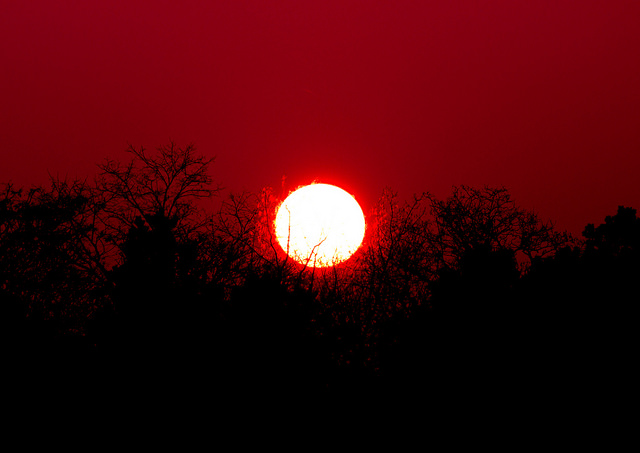
\includegraphics[width=0.5\linewidth]{images/SCP.001.when.night.breaks.jpg}
	\caption*{SCP-001激活后数分钟,拍摄者未知。}
\end{figure}

\bb{项目编号:}SCP-001

\bb{项目等级:}Apollyon

\bb{特殊收容措施:}\red{文件恢复于此前版本。信息崩溃。}

\bb{描述:}\red{文件恢复于此前版本。信息崩溃。}

\cl{\red{
+打开附件\\
...\\
...\\
...\\
授予访问权限
}}

\begin{scpbox}
Igotta博士出现在画面中,状态看起来比以前更加糟糕,头发明显稀疏,中间缺了大片。若不是正反射着显示器的柔和光芒,你甚至会以为她不再拥有双眼,因为它们已深陷入了她的眼窝之中。她眼睛一眨不眨地凝视着前方。
\end{scpbox}

\begin{scpdialog}
“她不会停止,她,她从未离去,我知道我没有,没有因浏览文档感染信息危害。我测试自己是否受到-4673感染,答案是否定的。-5189是,是唯一,唯一使用打印作为载体的,不 – 不是,我仍拥有全部的手指!”
\end{scpdialog}

\begin{scpbox}
她咧开双唇,露出一个破碎的笑容,她微弱地笑着,露出颤抖的双手,似乎曾是手指的骨骼遗骸大部分嵌入了她左手的血肉之中 – 支撑着她无名指处的残肢。两枚婚戒松散地套在上面,彼此相碰。
\end{scpbox}

\begin{scpdialog}
“所以,我没有感染,我不是,没有,我,我没有发疯。我知道,我知道仪式如何运转,我知道这真的是她,是她的,她——”
\end{scpdialog}

\begin{scpbox}
有些东西使她的注意力离开屏幕,她转首听着。
\end{scpbox}

\begin{scpdialog}
“不!不,我不 – 不能!你不是,不是你,这不一样。不是你,这再也不是你了,不!不不不!
\end{scpdialog}

\begin{scpbox}
她用力揉着自己的太阳穴,一遍又一遍地重复道。一分钟后,她转回头,面对摄像机。
\end{scpbox}

\begin{scpdialog}
“它是她又不是,我所带回的 – 仍然是一部分,没办法,束手无策,无可挽回。

未来对我来说毫无希望,上帝啊,我不能再这样下去了。

我在这儿很安全,光线无法到我身边 – 我,我不 – 不会让它,让它带走我。
\end{scpdialog}

\begin{scpbox}
她挥舞着一把手枪。
\end{scpbox}

\begin{scpdialog}
我本来计 – 计划用这个,直到我找到了剩下的,剩下的药物。我不想冒险,冒险将它们的注意力转移到我 - 我的身上……我的身体。
\end{scpdialog}

\begin{scpbox}
她拉开办公桌的抽屉,放好手枪,抬起眼皮凝视着摄像头。
\end{scpbox}

\begin{scpdialog}
妈妈,爸爸,Ari。

我很抱歉。”
\end{scpdialog}

\begin{scpbox}
她前倾身体,记录结束。
\end{scpbox}

\hr

\tred{太可怕了}

\tred{就这样结束了吗?}

\begin{scpbox}
你拉开抽屉,抽出手枪,心不在焉地在手里翻弄了一会儿,想知道你该到那里去。Site-17?64?当然你不会是最后的幸存者。电脑发出声响,文件有更新吗?
\end{scpbox}

\hr

\bb{项目编号:}

\cl{
\ii{炽日升上了藏红花似的天空\\
偶然地相逢,彼此不安地表现\\
终有一日,吾爱,我们二者将}
}

\bb{项目等级:}

\cl{
\ii{融为一体,进程就此开始\\
浓雾迷乱而狂野,闪耀光辉;\\
旭日的光芒四射于湛蓝的晴空}
}

\bb{特殊收容措施:}

\cl{
\ii{就在我们奋力奔跑之时\\
穿越隧道,狂野的热潮,\\
那日,吾爱,我们终将拥有}

\ii{共度的未来 – 我们所赢得的生活\\
承诺与责任,为我们组建的家庭\\
蔚蓝的天空埋葬了闪耀的}
}

\bb{描述:}

\cl{
\ii{阳光,被命运淹没 – 超支\\
愤怒与怨恨肆意滋生\\
昨日,吾爱,你我尚为一体}

\ii{此刻你静卧于此,你的生命已离去\\
徘徊于她射线外的黑暗\\
绯红的天幕在火炬下烧灼;我们的太阳,\\
今日,吾爱,我们融为一体}
}

\begin{figure}[H]
	\centering
	
\includegraphics[width=0.5\linewidth]{images/SCP.001.when.night.breaks.3.jpg}
	\caption*{系统错误误误误误误误误误\#@\&\#.}
\end{figure}

\hr

\begin{scpbox}

没有你的命令,显示器开始自动播放视频文件,当你看到加载出的图像时,寒意涌上心头。

这是一幕实时录像,来自你的背后,距离大约一英尺远。

一只骨瘦如柴的墨色左手进入画面,极缓慢地接近你。它没有无名指。

再来不及思考更多,你疯狂的转过身来举枪射击,希望能驱散幽灵。

你的子弹射入一面空荡荡的墙壁,此处一无所有。

在你听到它之前,有什么东西再度经过 – 在你听到它们的声音之前。流淌着的湿润的抨击伴随着尖声合唱涌入走廊。

它撞击着屋门,此处莫不是藏身之所?

它再度撞击,似乎有一张脸浮现出来,某一部分属于人类,其余部分则……是某些东西 - 正从缝隙中缓慢灌入。血肉从神知道由何而来的淤泥中渗出,重新组合成手指、眼睛与羽毛。

第三次。它此刻正压在木梁上,沉甸甸地使之向内下垂。

伴随着呻吟与破裂声,木梁支离破碎,门打开了。

手掌和臂膊拉起你,一个接一个地将你传递出去,经由空的收容单元,继续向上,穿过楼梯间,通往大厅和隧道。

你所拥有的宝贵黑暗不过片刻。

隧道的尽头,有光。

\end{scpbox}